\documentclass[]{article}
\usepackage{lmodern}
\usepackage{amssymb,amsmath}
\usepackage{ifxetex,ifluatex}
\usepackage{fixltx2e} % provides \textsubscript
\ifnum 0\ifxetex 1\fi\ifluatex 1\fi=0 % if pdftex
  \usepackage[T1]{fontenc}
  \usepackage[utf8]{inputenc}
\else % if luatex or xelatex
  \ifxetex
    \usepackage{mathspec}
  \else
    \usepackage{fontspec}
  \fi
  \defaultfontfeatures{Ligatures=TeX,Scale=MatchLowercase}
\fi
% use upquote if available, for straight quotes in verbatim environments
\IfFileExists{upquote.sty}{\usepackage{upquote}}{}
% use microtype if available
\IfFileExists{microtype.sty}{%
\usepackage{microtype}
\UseMicrotypeSet[protrusion]{basicmath} % disable protrusion for tt fonts
}{}
\usepackage[margin=1in]{geometry}
\usepackage{hyperref}
\PassOptionsToPackage{usenames,dvipsnames}{color} % color is loaded by hyperref
\hypersetup{unicode=true,
            pdftitle={Module 4: Recommended Exercises},
            pdfauthor={Martina Hall, Michail Spitieris, Stefanie Muff, Department of Mathematical Sciences, NTNU},
            colorlinks=true,
            linkcolor=Maroon,
            citecolor=Blue,
            urlcolor=blue,
            breaklinks=true}
\urlstyle{same}  % don't use monospace font for urls
\usepackage{color}
\usepackage{fancyvrb}
\newcommand{\VerbBar}{|}
\newcommand{\VERB}{\Verb[commandchars=\\\{\}]}
\DefineVerbatimEnvironment{Highlighting}{Verbatim}{commandchars=\\\{\}}
% Add ',fontsize=\small' for more characters per line
\usepackage{framed}
\definecolor{shadecolor}{RGB}{248,248,248}
\newenvironment{Shaded}{\begin{snugshade}}{\end{snugshade}}
\newcommand{\KeywordTok}[1]{\textcolor[rgb]{0.13,0.29,0.53}{\textbf{#1}}}
\newcommand{\DataTypeTok}[1]{\textcolor[rgb]{0.13,0.29,0.53}{#1}}
\newcommand{\DecValTok}[1]{\textcolor[rgb]{0.00,0.00,0.81}{#1}}
\newcommand{\BaseNTok}[1]{\textcolor[rgb]{0.00,0.00,0.81}{#1}}
\newcommand{\FloatTok}[1]{\textcolor[rgb]{0.00,0.00,0.81}{#1}}
\newcommand{\ConstantTok}[1]{\textcolor[rgb]{0.00,0.00,0.00}{#1}}
\newcommand{\CharTok}[1]{\textcolor[rgb]{0.31,0.60,0.02}{#1}}
\newcommand{\SpecialCharTok}[1]{\textcolor[rgb]{0.00,0.00,0.00}{#1}}
\newcommand{\StringTok}[1]{\textcolor[rgb]{0.31,0.60,0.02}{#1}}
\newcommand{\VerbatimStringTok}[1]{\textcolor[rgb]{0.31,0.60,0.02}{#1}}
\newcommand{\SpecialStringTok}[1]{\textcolor[rgb]{0.31,0.60,0.02}{#1}}
\newcommand{\ImportTok}[1]{#1}
\newcommand{\CommentTok}[1]{\textcolor[rgb]{0.56,0.35,0.01}{\textit{#1}}}
\newcommand{\DocumentationTok}[1]{\textcolor[rgb]{0.56,0.35,0.01}{\textbf{\textit{#1}}}}
\newcommand{\AnnotationTok}[1]{\textcolor[rgb]{0.56,0.35,0.01}{\textbf{\textit{#1}}}}
\newcommand{\CommentVarTok}[1]{\textcolor[rgb]{0.56,0.35,0.01}{\textbf{\textit{#1}}}}
\newcommand{\OtherTok}[1]{\textcolor[rgb]{0.56,0.35,0.01}{#1}}
\newcommand{\FunctionTok}[1]{\textcolor[rgb]{0.00,0.00,0.00}{#1}}
\newcommand{\VariableTok}[1]{\textcolor[rgb]{0.00,0.00,0.00}{#1}}
\newcommand{\ControlFlowTok}[1]{\textcolor[rgb]{0.13,0.29,0.53}{\textbf{#1}}}
\newcommand{\OperatorTok}[1]{\textcolor[rgb]{0.81,0.36,0.00}{\textbf{#1}}}
\newcommand{\BuiltInTok}[1]{#1}
\newcommand{\ExtensionTok}[1]{#1}
\newcommand{\PreprocessorTok}[1]{\textcolor[rgb]{0.56,0.35,0.01}{\textit{#1}}}
\newcommand{\AttributeTok}[1]{\textcolor[rgb]{0.77,0.63,0.00}{#1}}
\newcommand{\RegionMarkerTok}[1]{#1}
\newcommand{\InformationTok}[1]{\textcolor[rgb]{0.56,0.35,0.01}{\textbf{\textit{#1}}}}
\newcommand{\WarningTok}[1]{\textcolor[rgb]{0.56,0.35,0.01}{\textbf{\textit{#1}}}}
\newcommand{\AlertTok}[1]{\textcolor[rgb]{0.94,0.16,0.16}{#1}}
\newcommand{\ErrorTok}[1]{\textcolor[rgb]{0.64,0.00,0.00}{\textbf{#1}}}
\newcommand{\NormalTok}[1]{#1}
\usepackage{graphicx,grffile}
\makeatletter
\def\maxwidth{\ifdim\Gin@nat@width>\linewidth\linewidth\else\Gin@nat@width\fi}
\def\maxheight{\ifdim\Gin@nat@height>\textheight\textheight\else\Gin@nat@height\fi}
\makeatother
% Scale images if necessary, so that they will not overflow the page
% margins by default, and it is still possible to overwrite the defaults
% using explicit options in \includegraphics[width, height, ...]{}
\setkeys{Gin}{width=\maxwidth,height=\maxheight,keepaspectratio}
\IfFileExists{parskip.sty}{%
\usepackage{parskip}
}{% else
\setlength{\parindent}{0pt}
\setlength{\parskip}{6pt plus 2pt minus 1pt}
}
\setlength{\emergencystretch}{3em}  % prevent overfull lines
\providecommand{\tightlist}{%
  \setlength{\itemsep}{0pt}\setlength{\parskip}{0pt}}
\setcounter{secnumdepth}{0}
% Redefines (sub)paragraphs to behave more like sections
\ifx\paragraph\undefined\else
\let\oldparagraph\paragraph
\renewcommand{\paragraph}[1]{\oldparagraph{#1}\mbox{}}
\fi
\ifx\subparagraph\undefined\else
\let\oldsubparagraph\subparagraph
\renewcommand{\subparagraph}[1]{\oldsubparagraph{#1}\mbox{}}
\fi

%%% Use protect on footnotes to avoid problems with footnotes in titles
\let\rmarkdownfootnote\footnote%
\def\footnote{\protect\rmarkdownfootnote}

%%% Change title format to be more compact
\usepackage{titling}

% Create subtitle command for use in maketitle
\providecommand{\subtitle}[1]{
  \posttitle{
    \begin{center}\large#1\end{center}
    }
}

\setlength{\droptitle}{-2em}

  \title{Module 4: Recommended Exercises}
    \pretitle{\vspace{\droptitle}\centering\huge}
  \posttitle{\par}
  \subtitle{TMA4268 Statistical Learning V2020}
  \author{Martina Hall, Michail Spitieris, Stefanie Muff, Department of
Mathematical Sciences, NTNU}
    \preauthor{\centering\large\emph}
  \postauthor{\par}
      \predate{\centering\large\emph}
  \postdate{\par}
    \date{January 30, 2020}


\begin{document}
\maketitle

\section{Theoretical exercises}\label{theoretical-exercises}

\subsection{Problem 1: KNN (Exercise 2.4.7 in ISL textbook slightly
modified)}\label{problem-1-knn-exercise-2.4.7-in-isl-textbook-slightly-modified}

The table and plot below provides a training data set consisting of
seven observations, two predictors and one qualitative response
variable.

\begin{verbatim}
##   x1 x2 y
## 1  3  3 A
## 2  2  0 A
## 3  1  1 A
## 4  0  1 B
## 5 -1  0 B
## 6  2  1 B
## 7  1  0 B
\end{verbatim}

\begin{center}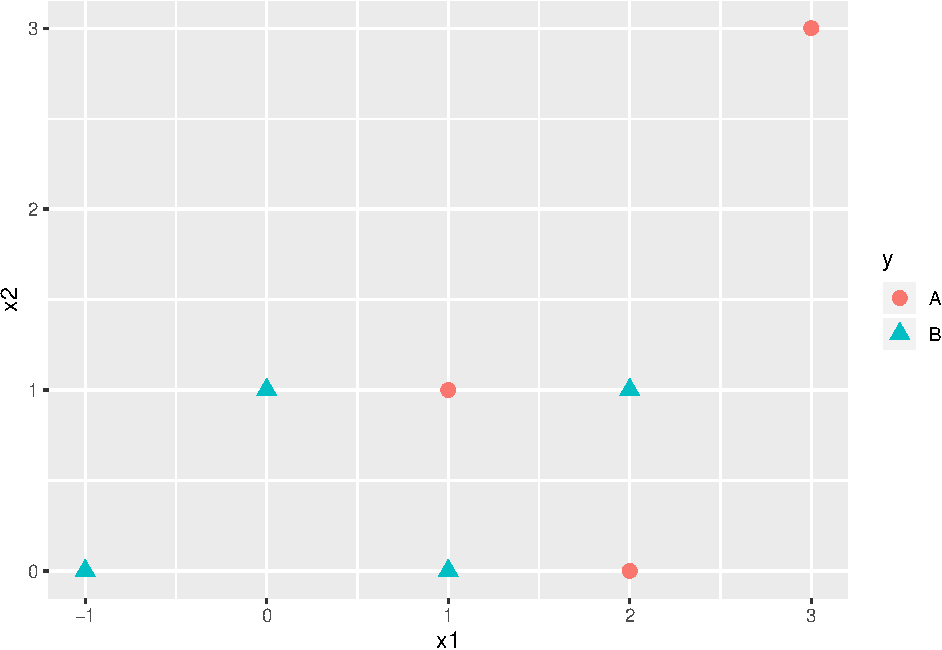
\includegraphics[width=0.7\linewidth]{RecEx4_files/figure-latex/unnamed-chunk-1-1} \end{center}

We wish to use this data set to make a prediction for \(Y\) when
\(X_1=1, X_2=2\) using the \(K\)-nearest neighbors classification
method.

\begin{enumerate}
\def\labelenumi{\alph{enumi}.}
\tightlist
\item
  Calculate the Euclidean distance between each observation and the test
  point, \(X_1=1,X_2=2\).
\item
  Use \(P(Y=j|X=x_0) = \frac{1}{K}\sum_{I \in \mathcal{N}_0}I(Y=j)\) to
  predict the class of \(Y\) when \(K=1\), \(K=4\) and \(K=7\). Why is
  \(K=7\) a bad choise?
\item
  If the Bayes decision boundary in this problem is highly non-linear,
  would we expect the best value for \(K\) to be large or small? Why?
\end{enumerate}

\subsection{Problem 2: Bank notes and LDA (with
calculations)}\label{problem-2-bank-notes-and-lda-with-calculations}

To distinguish between genuine and fake bank notes measurements of
length and diagonal of an image part of the bank notes have been
performed. For 1000 bank notes (500 of each of genuine and false) this
gave the following values for the mean and the covariance matrix (using
unbiased estimators), where the first value is the length of the bank
note.

Genuine bank notes: \[
   \bar{\bf x}_G=\left[     \begin{array}{c} 214.97 \\ 141.52  \end{array} \right]
\text{ and }
   \hat{\boldsymbol \Sigma}_G=\left[     \begin{array}{cc} 0.1502 & 0.0055 \\ 0.0055 & 0.1998 
\end{array} \right]
\]

Fake bank notes: \[
   \bar{\bf x}_F= \left[     \begin{array}{c} 214.82 \\ 139.45  \end{array} \right]
\text{ and }
   \hat{\boldsymbol \Sigma}_F= \left[     \begin{array}{cc} 0.1240 & 0.0116 \\ 0.0116 & 0.3112 
\end{array} \right]
\]

\begin{enumerate}
\def\labelenumi{\alph{enumi}.}
\item
  Assume the true covariance matrix for the genuine and fake bank notes
  are the same. How would you estimate the common covariance matrix?
\item
  Explain the assumptions made to use linear discriminant analysis to
  classify a new observation to be a genuine or a fake bank note. Write
  down the classification rule for a new observation (make any
  assumptions you need to make).
\item
  Use the method in b. to determine if a bank note with length 214.0 and
  diagonal 140.4 is genuine or fake. You can use R to perform the matrix
  calculations.
\end{enumerate}

\textbf{R-hints}:

\begin{Shaded}
\begin{Highlighting}[]
\CommentTok{# inv(A)}
\KeywordTok{solve}\NormalTok{(A)}
\CommentTok{# transpose of vector}
\KeywordTok{t}\NormalTok{(v)}
\CommentTok{# determinant of A}
\KeywordTok{det}\NormalTok{(A)}
\CommentTok{# multiply vector and matrix/ matrix and matrix}
\NormalTok{v }\OperatorTok\StringTok{ }\NormalTok{A}
\NormalTok{B }\OperatorTok\StringTok{ }\NormalTok{A}
\end{Highlighting}
\end{Shaded}

\begin{enumerate}
\def\labelenumi{\alph{enumi}.}
\setcounter{enumi}{3}
\tightlist
\item
  What is the difference between LDA and QDA? Use the classification
  rule for QDA to determine the bank note from c. Do you obtain the same
  result? (You can use R to perform the matrix calculations)
\end{enumerate}

Hint: the following formulas might be useful. \[A^{-1} = \left[
\begin{array}{cc} a & b \\ c & d \end{array} 
\right]^{-1} = \frac{1}{ad-bc}
\left[
\begin{array}{cc} d & -b \\ -c & a \end{array} 
\right]\]

\[ |A| = det(A) = \Big|\begin{array}{cc} a & b \\ c & d \end{array}\Big| = ad - bc \]

\subsection{Problem 3: Odds (Exercise 4.7.9 in ISL
textbook)}\label{problem-3-odds-exercise-4.7.9-in-isl-textbook}

This problem has to do with \emph{odds}.

\begin{enumerate}
\def\labelenumi{\alph{enumi}.}
\tightlist
\item
  On average, what fraction of people with an odds of 0.37 of defaulting
  on their credit card payment will in fact default?\\
\item
  Suppose that an individual has a 16\% chance of defaulting on her
  credit card payment. What are the odds that she will default?
\end{enumerate}

\subsection{Problem 4: Logistic regression (Exercise 4.7.6 in ISL
textbook)}\label{problem-4-logistic-regression-exercise-4.7.6-in-isl-textbook}

Suppose we collect data for a group of students in a statistics class
with variables \(x_1\) = hours studied, \(x_2\) = undergrad grade point
average (GPA), and \(Y\) = receive an A. We fit a logistic regression
and produce estimated coefficient,
\(\hat{\beta}_0 = -6, \hat{\beta}_1 = 0.05, \hat{\beta}_2 = 1\).

\begin{enumerate}
\def\labelenumi{\alph{enumi}.}
\tightlist
\item
  Estimate the probability that a student who studies for 40 h and has
  an undergrad GPA of 3.5 gets an A in the class.\\
\item
  How many hours would the student in part a. need to study to have a
  50\% probability of getting an A in the class?
\end{enumerate}

\subsection{Problem 5: Sensitivity, specificity, ROC and
AUC}\label{problem-5-sensitivity-specificity-roc-and-auc}

We have a two-class problem, with classes 0=non-disease and 1=disease,
and a method \(p(x)\) that produces probability of disease for a
covariate \(x\). In a population we have investigated \(N\) individuals
and know the predicted probability of disease \(p(x)\) and true disease
status for these \(N\).

\begin{enumerate}
\def\labelenumi{\alph{enumi}.}
\tightlist
\item
  We choose the rule \(p(x)>0.5\) to classify to disease. Define the
  sensitivity and the specificity of the test.
\item
  Explain how you can construct a reciever operator curve (ROC) for your
  setting, and why that is a useful thing to do. In particular, why do
  we want to investigate different cut-offs of the probability of
  disease?
\item
  Assume that we have a competing method \(q(x)\) that also produces
  probability of disease for a covariate \(x\). We get the information
  that the AUC of the \(p(x)\)-method is 0.6 and the AUC of the
  \(q(x)\)-method is 0.7. What is the definition and interpretation of
  the AUC? Would you prefer the \(p(x)\) or the \(q(x)\) method for
  classification?
\end{enumerate}

\section{Data analysis with R}\label{data-analysis-with-r}

For the following problems, you should check out and learn how to use
the following R functions: \texttt{glm()} (\texttt{stats} library),
\texttt{lda()}, \texttt{qda()} (\texttt{MASS} library), \texttt{knn()}
(\texttt{class} library), \texttt{roc()} and \texttt{auc()}
(\texttt{pROC} library).

\subsection{Problem 6 (Exercise 4.7.10 in ISL textbook -
modified)}\label{problem-6-exercise-4.7.10-in-isl-textbook---modified}

This question should be answered using the \texttt{Weekly} data set,
which is part of the \texttt{ISLR} packages. This data is similar in
nature to the \texttt{Smarket} data from this chapter's lab, except that
it contains 1,089 weekly returns for 21 years, from the beginning of
1990 to the end of 2010.

\begin{enumerate}
\def\labelenumi{\alph{enumi}.}
\tightlist
\item
  Produce numerical and graphical summaries of the \texttt{Weekly} data.
  Do there appear to be any patterns? \textbf{R-hint}: Load the data as
  follows:
\end{enumerate}

\begin{Shaded}
\begin{Highlighting}[]
\KeywordTok{attach}\NormalTok{(Weekly)}
\end{Highlighting}
\end{Shaded}

\begin{enumerate}
\def\labelenumi{\alph{enumi}.}
\setcounter{enumi}{1}
\item
  Use the full data set to perform a logistic regression with
  \texttt{Direction} as the response and the five lag variables plus
  \texttt{Volume} as predictors. Use the \texttt{summary()} function to
  print the results. Which of these predictors appears to be of
  interest?\\
  \textbf{R-hints:} You should use the \texttt{glm()} function with the
  argument \texttt{family="binomial"} to make a logistic regression
  model.
\item
  Compute the confusion matrix and overall fraction of correct
  predictions. Explain what the confusion matrix is telling you about
  the types of mistakes made by logistic regression.\\
  \textbf{R-hints:} insert the name of your model for
  \texttt{yourGlmModel} in the code below to get the predicted
  probabilities for ``Up'', the classified direction and the confusion
  matrix.
\end{enumerate}

\begin{Shaded}
\begin{Highlighting}[]
\NormalTok{glm.probs_Weekly =}\StringTok{ }\KeywordTok{predict}\NormalTok{(yourGlmModel, }\DataTypeTok{type =} \StringTok{"response"}\NormalTok{)}
\NormalTok{glm.preds_Weekly =}\StringTok{ }\KeywordTok{ifelse}\NormalTok{(glm.probs_Weekly }\OperatorTok{>}\StringTok{ }\FloatTok{0.5}\NormalTok{, }\StringTok{"Up"}\NormalTok{, }\StringTok{"Down"}\NormalTok{)}
\KeywordTok{table}\NormalTok{(glm.preds_Weekly, Direction)}
\end{Highlighting}
\end{Shaded}

\begin{enumerate}
\def\labelenumi{\alph{enumi}.}
\setcounter{enumi}{3}
\tightlist
\item
  Now fit the logistic regression model using a training data period
  from 1990 to 2008, with \texttt{Lag2} as the only predictor. Compute
  the confusion matrix and the overall fraction of correct predictions
  for the held out data (that is, the data from 2009 and 2010).\\
  \textbf{R-hints:} use the following code to divide into test and train
  set. For predicting the direction of the test set, use
  \texttt{newdata\ =\ Weekly\_test} in the \texttt{predict()} function.
\end{enumerate}

\begin{Shaded}
\begin{Highlighting}[]
\NormalTok{Weekly_trainID =}\StringTok{ }\NormalTok{(Year }\OperatorTok{<}\StringTok{ }\DecValTok{2009}\NormalTok{)}
\NormalTok{Weekly_train =}\StringTok{ }\NormalTok{Weekly[Weekly_trainID, ]}
\NormalTok{Weekly_test =}\StringTok{ }\NormalTok{Weekly[}\OperatorTok{!}\NormalTok{Weekly_trainID, ]}
\end{Highlighting}
\end{Shaded}

\begin{enumerate}
\def\labelenumi{\alph{enumi}.}
\setcounter{enumi}{4}
\tightlist
\item
  Repeat d) using LDA.
\item
  Repeat d) using QDA.
\end{enumerate}

\textbf{R-hints:} plug in you variables in the following code to perform
lda and qda (just replacing \texttt{lda} with \texttt{qda}).

\begin{Shaded}
\begin{Highlighting}[]
\KeywordTok{library}\NormalTok{(MASS)}
\NormalTok{lda.Weekly =}\StringTok{ }\KeywordTok{lda}\NormalTok{(Response }\OperatorTok{~}\StringTok{ }\NormalTok{pred1, }\DataTypeTok{data =}\NormalTok{ youTrainData)}
\NormalTok{lda.Weekly_pred =}\StringTok{ }\KeywordTok{predict}\NormalTok{(yourModel, }\DataTypeTok{newdata =}\NormalTok{ YourTestData)}\OperatorTok{$}\NormalTok{class}
\NormalTok{lda.Weekly_prob =}\StringTok{ }\KeywordTok{predict}\NormalTok{(yourModel, }\DataTypeTok{newdata =}\NormalTok{ YourTestData)}\OperatorTok{$}\NormalTok{posterior}
\KeywordTok{table}\NormalTok{(lda.Weekly_pred, YourTestData}\OperatorTok{$}\NormalTok{Direction)}
\end{Highlighting}
\end{Shaded}

\begin{enumerate}
\def\labelenumi{\alph{enumi}.}
\setcounter{enumi}{6}
\tightlist
\item
  Repeat d) using KNN with \(K=1\).
\end{enumerate}

\textbf{R-hints:} plug in you variables in the following code to perform
KNN. The argument \texttt{prob=T} will provide the probabilities for the
classified direction (which you will need later). When there are ties
(same amount of Up and Down for the nearest neighbors), the \texttt{knn}
function picks a class at random. We use the \texttt{set.seed()}
function such that we don't get different answers for each time we run
the code.

\begin{Shaded}
\begin{Highlighting}[]
\KeywordTok{library}\NormalTok{(class)}
\NormalTok{knn.train =}\StringTok{ }\KeywordTok{as.matrix}\NormalTok{(YourTrainData}\OperatorTok{$}\NormalTok{Lag2)}
\NormalTok{knn.test =}\StringTok{ }\KeywordTok{as.matrix}\NormalTok{(YourTestData}\OperatorTok{$}\NormalTok{Lag2)}

\KeywordTok{set.seed}\NormalTok{(}\DecValTok{123}\NormalTok{)}
\NormalTok{yourKNNmodel =}\StringTok{ }\KeywordTok{knn}\NormalTok{(}\DataTypeTok{train =}\NormalTok{ knn.train, }\DataTypeTok{test =}\NormalTok{ knn.test, }\DataTypeTok{cl =}\NormalTok{ YourTrainData}\OperatorTok{$}\NormalTok{Direction, }
    \DataTypeTok{k =}\NormalTok{ YourValueOfK, }\DataTypeTok{prob =}\NormalTok{ T)}
\KeywordTok{table}\NormalTok{(yourKNNmodel, YourTestData}\OperatorTok{$}\NormalTok{Direction)}
\end{Highlighting}
\end{Shaded}

\begin{enumerate}
\def\labelenumi{\alph{enumi}.}
\setcounter{enumi}{7}
\tightlist
\item
  Use the following code to find the best value of \(K\). Report the
  confusion matrix and overall fraction of correct predictions for this
  value of \(K\).
\end{enumerate}

\begin{Shaded}
\begin{Highlighting}[]
\CommentTok{# knn error:}
\NormalTok{K =}\StringTok{ }\DecValTok{30}
\NormalTok{knn.error =}\StringTok{ }\KeywordTok{rep}\NormalTok{(}\OtherTok{NA}\NormalTok{, K)}

\KeywordTok{set.seed}\NormalTok{(}\DecValTok{234}\NormalTok{)}
\ControlFlowTok{for}\NormalTok{ (k }\ControlFlowTok{in} \DecValTok{1}\OperatorTok{:}\NormalTok{K) \{}
\NormalTok{    knn.pred =}\StringTok{ }\KeywordTok{knn}\NormalTok{(}\DataTypeTok{train =}\NormalTok{ knn.train, }\DataTypeTok{test =}\NormalTok{ knn.test, }\DataTypeTok{cl =}\NormalTok{ Weekly_train}\OperatorTok{$}\NormalTok{Direction, }
        \DataTypeTok{k =}\NormalTok{ k)}
\NormalTok{    knn.error[k] =}\StringTok{ }\KeywordTok{mean}\NormalTok{(knn.pred }\OperatorTok{!=}\StringTok{ }\NormalTok{Weekly_test}\OperatorTok{$}\NormalTok{Direction)}
\NormalTok{\}}
\NormalTok{knn.error.df =}\StringTok{ }\KeywordTok{data.frame}\NormalTok{(}\DataTypeTok{k =} \DecValTok{1}\OperatorTok{:}\NormalTok{K, }\DataTypeTok{error =}\NormalTok{ knn.error)}
\KeywordTok{ggplot}\NormalTok{(knn.error.df, }\KeywordTok{aes}\NormalTok{(}\DataTypeTok{x =}\NormalTok{ k, }\DataTypeTok{y =}\NormalTok{ error)) }\OperatorTok{+}\StringTok{ }\KeywordTok{geom_point}\NormalTok{(}\DataTypeTok{col =} \StringTok{"blue"}\NormalTok{) }\OperatorTok{+}\StringTok{ }\KeywordTok{geom_line}\NormalTok{(}\DataTypeTok{linetype =} \StringTok{"dotted"}\NormalTok{)}
\end{Highlighting}
\end{Shaded}

\begin{enumerate}
\def\labelenumi{\roman{enumi}.}
\tightlist
\item
  Which of these methods appear to provide the best results on this
  data?
\end{enumerate}

\begin{enumerate}
\def\labelenumi{\alph{enumi}.}
\setcounter{enumi}{9}
\tightlist
\item
  Plot the ROC curves and calculate the AUC for the four methods (using
  your the best choice for KNN). What can you say about the fit of these
  models?
\end{enumerate}

\textbf{R-hints}:

\begin{itemize}
\tightlist
\item
  For KNN you can use \texttt{knn(...,prob=TRUE)} to get the probability
  for the classified direction. Note that we want \(P(Direction = Up)\)
  when plotting the ROC-curve, so we need to modify the probabilties
  returned from the \texttt{knn} function.
\end{itemize}

\begin{Shaded}
\begin{Highlighting}[]
\CommentTok{# get the probabilities for the classified class}
\NormalTok{yourKNNProbs =}\StringTok{ }\KeywordTok{attributes}\NormalTok{(yourKNNmodel)}\OperatorTok{$}\NormalTok{prob}

\CommentTok{# since we want the probability for Up, we need to take 1-p for the elements}
\CommentTok{# that gives probability for Down}
\NormalTok{down =}\StringTok{ }\KeywordTok{which}\NormalTok{(yourKNNmodel }\OperatorTok{==}\StringTok{ "Down"}\NormalTok{)}
\NormalTok{yourKNNProbs[down] =}\StringTok{ }\DecValTok{1} \OperatorTok{-}\StringTok{ }\NormalTok{yourKNNProbs[down]}
\end{Highlighting}
\end{Shaded}

\begin{itemize}
\tightlist
\item
  Use the following code to produce ROC-curves
\end{itemize}

\begin{Shaded}
\begin{Highlighting}[]
\CommentTok{# install.packages('plotROC') install.packages('pROC')}
\KeywordTok{library}\NormalTok{(pROC)}
\KeywordTok{library}\NormalTok{(plotROC)}

\NormalTok{yourRoc =}\StringTok{ }\KeywordTok{roc}\NormalTok{(}\DataTypeTok{response =}\NormalTok{ Weekly_test}\OperatorTok{$}\NormalTok{Direction, }\DataTypeTok{predictor =}\NormalTok{ yourModelsPredictedProb)}
\CommentTok{# you can use this function for all your methods and plot them using}
\CommentTok{# plot(yourRoc)}

\CommentTok{# or use ggplot2}
\NormalTok{dat =}\StringTok{ }\KeywordTok{data.frame}\NormalTok{(}\DataTypeTok{Direction =}\NormalTok{ Weekly_test}\OperatorTok{$}\NormalTok{Direction, }\DataTypeTok{glm =}\NormalTok{ yourGlmProbs, }\DataTypeTok{lda =}\NormalTok{ yourLDAProbs[, }
    \DecValTok{2}\NormalTok{], }\DataTypeTok{qda =}\NormalTok{ yourQDAProbs[, }\DecValTok{2}\NormalTok{], }\DataTypeTok{knn =}\NormalTok{ yourKNNProbs)}
\NormalTok{dat_long =}\StringTok{ }\KeywordTok{melt_roc}\NormalTok{(dat, }\StringTok{"Direction"}\NormalTok{, }\KeywordTok{c}\NormalTok{(}\StringTok{"glm"}\NormalTok{, }\StringTok{"lda"}\NormalTok{, }\StringTok{"qda"}\NormalTok{, }\StringTok{"knn"}\NormalTok{))}
\KeywordTok{ggplot}\NormalTok{(dat_long, }\KeywordTok{aes}\NormalTok{(}\DataTypeTok{d =}\NormalTok{ D, }\DataTypeTok{m =}\NormalTok{ M, }\DataTypeTok{color =}\NormalTok{ name)) }\OperatorTok{+}\StringTok{ }\KeywordTok{geom_roc}\NormalTok{(}\DataTypeTok{n.cuts =}\NormalTok{ F) }\OperatorTok{+}\StringTok{ }\KeywordTok{xlab}\NormalTok{(}\StringTok{"1-Specificity"}\NormalTok{) }\OperatorTok{+}\StringTok{ }
\StringTok{    }\KeywordTok{ylab}\NormalTok{(}\StringTok{"Sensitivity"}\NormalTok{)}
\CommentTok{# glm is very similar to lda, so the roc-curve for glm is not shown.}


\CommentTok{# AUC: yourAUC = auc(yourRoc)}
\end{Highlighting}
\end{Shaded}


\end{document}
